\documentclass[a4paper, 12pt]{article}
\usepackage[margin=1in]{geometry}
\usepackage[english]{babel}
\usepackage[utf8]{inputenc}
\usepackage{tcolorbox}
\usepackage{listings}
\usepackage{color, soul}
\usepackage{xcolor}
\usepackage{amsmath}
\usepackage{mathtools}
\usepackage{graphicx}
\usepackage{textcomp}
\usepackage{url}
\tcbuselibrary{breakable}

%% MATLAB
\definecolor{codegreen}{rgb}{0,0.6,0}
\definecolor{codegray}{rgb}{0.5,0.5,0.5}
\definecolor{codepurple}{rgb}{0.58,0,0.82}
\definecolor{backcolour}{rgb}{0.95,0.95,0.92}

\lstdefinestyle{mystyle}{
	backgroundcolor = \color{backcolour},
	commentstyle = \color{codegreen},
	keywordstyle = \color{magenta},
	numberstyle = \tiny\color{codegray},
	stringstyle=\color{codepurple},
	basicstyle=\ttfamily\footnotesize,
	breakatwhitespace=false,
	breaklines=true,
	captionpos = b,
	keepspaces = true,
	numbers = left,
	numbersep = 5pt,
	showspaces = false,
	showstringspaces = false,
	showtabs = false,
	tabsize = 2
}

\lstset{style=mystyle}

%%%

\begin{document}
\title{BRI509: Introduction to Brain Signal Processing \\ Assignment No. 4}
\author{\underline{\textbf{CANOY RAYMART JAY}} \\ Student ID \#: \underline{\textbf{2020021376}}}
\date{\today}
\maketitle

\begin{itemize}
\item[\textbf{1}]{Explain the following terms briefly.}

\begin{itemize}
\item[(a)]{Sampling theorem}
The process of sampling involves multiplying the original signal by a pulse train, with each pulse having an area of one, that is,

\begin{figure}[h!]
\center{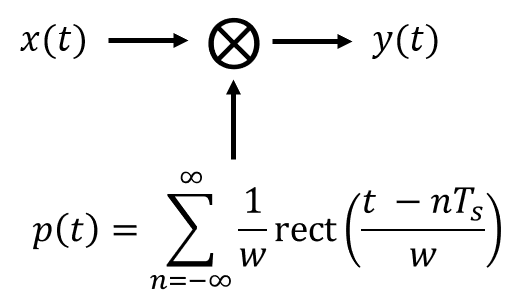
\includegraphics[width=5cm]{sampling_theorem.png}}
\caption{\label{fig:sampling_theorem} The sampling process}
\end{figure}

Therefore, 
\begin{equation}
y(t) = \sum_{n=-\infty}^{+\infty}{x(t) \frac{1}{w} \mathtt{rect}\left( \frac{t - nT_{s}}{w}\right)}.
\end{equation}

To get the original value of the signal, the width of the pulse should approach zero:

\begin{equation}
\begin{gathered}
\begin{alignedat}{1}
x_{\delta}(t) &= \lim_{w \to 0}  \sum_{n=-\infty}^{+\infty}{x(t) \frac{1}{w} \mathtt{rect}\left( \frac{t - nT_{s}}{w}\right)}, \\
x_{\delta}(t) &= \sum_{n=-\infty}^{+\infty}{x(t) \delta \left(t - nT_{s}\right)}
\end{alignedat}
\end{gathered}
\end{equation}

By taking the CTFT of this impulse-sampled signal, we get
\begin{equation}
\begin{gathered}
\begin{alignedat}{1}
X(f) & = \sum_{n=-\infty}^{+\infty} {X(f) f_{s}\delta \left(f - nf_{s} \right)}, \\
X(f) & = f_{s} X(f) \ast \delta_{f_{s}}(f)
\end{alignedat}
\end{gathered}
\end{equation}

The CTFT of this impulse-sampled signal is just the replicas (aliases) of the CTFT of the original signal. The idea in sampling theorem is that the signal should be bandlimited, which means that the non-zero values should be confined to a finite range of frequency, so that the original signal could be recovered from the samples when a filter is applied.

\item[(b)]{Anti-aliasing}
Aliasing is the phenomenon where the aliases (replicas of the CTFT of the original signal) overlap with each other. To avoid aliasing, the sampling rate $f_{s}$ should be greater than twice the highest frequency $f_{m}$ in a lowpass bandlimited signal. But more generally, the minimum sampling rate should be
\begin{equation}
|f_{s, \mathtt{min}}| > \frac{2f_{H}}{[f_{H}/B]},
\end{equation}
where $f_{H}$ and $f_{L}$ are the highest and lowest frequencies, respectively, in the finite range where the CTFT of the original signal is non zero. $B$ is the bandwidth of the CTFT, i.e., $B = f_{H} - f_{L}$.

\item[(c)]{Bandlimited signal}
Bandlimited signals are signals which are zero for all values greater than the highest frequency $f_{m}$. 

\begin{figure}[h!]
\center{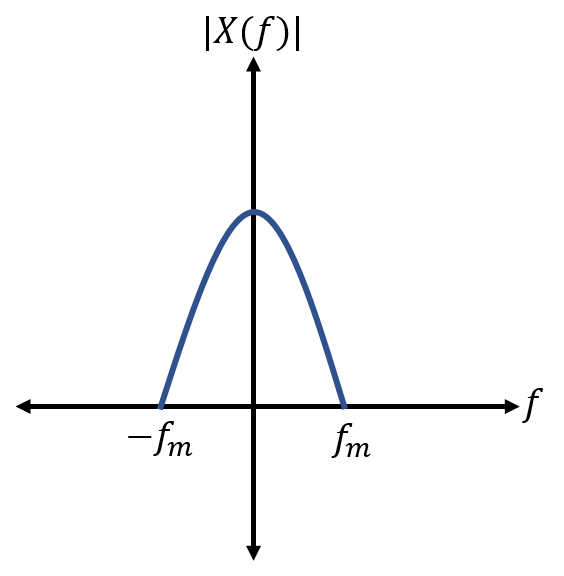
\includegraphics[width=5cm]{lowpass_bandlimited_signal.png}}
\caption{\label{fig:lowpass}Lowpass bandlimited signal.}
\end{figure}


\begin{figure}[h!]
\center{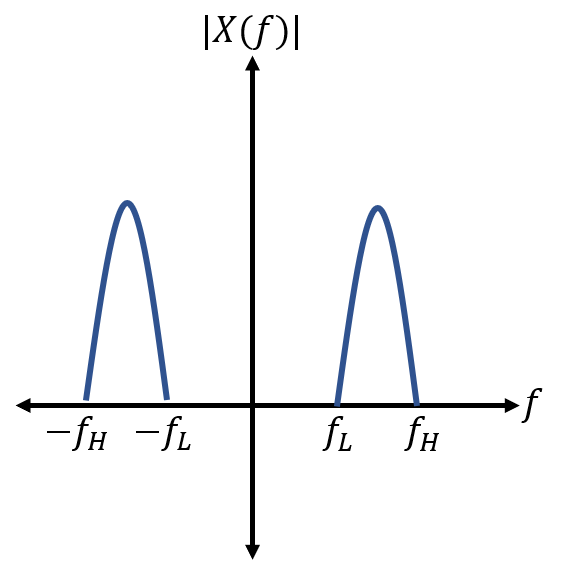
\includegraphics[width=5cm]{bandlimited_signal.png}}
\caption{\label{fig:lowpass}Bandlimited signal with a bandwidth of $B = |f_{H}| - |f_{L}|$.}
\end{figure}

\item[(d)]{Distortion}
Distortion is a phenomenon where the shape of the signal is being changed when a filter is used. It should be noted, however, that the multiplication of a signal by a constant and the time shifts are not considered as distortion.

\item[(e)]{Causal filters}
Causal filters are filters with nonzero response only after the impulse is applied at time $t = 0$.

\item[(f)]{Linear phase}
The impulse response of a distortionless system can be generally described as 

\begin{equation}
h(t) = A\delta (t - t_{0}),
\end{equation}

and its CTFT can be written as 
\begin{equation}
H(f) = A e^{-j 2 \pi f t_{0}}.
\end{equation}
This frequency responses has a constant magnitude and a linear phase, that is, $|H(f)| = A$ and $\angle H(f) = 2 \pi f t_{0}$. 
\end{itemize}

\item[\textbf{2}]{Solve the following problems.}

\begin{itemize}
\item[(a)]{Draw a cascade-form block diagram for the system transfer function.}
\begin{equation}
H(z) = \frac{z}{(z + 1/3)(z - 3/4)}
\end{equation}

\textbf{Solution:}
\begin{figure}[h!]
\center{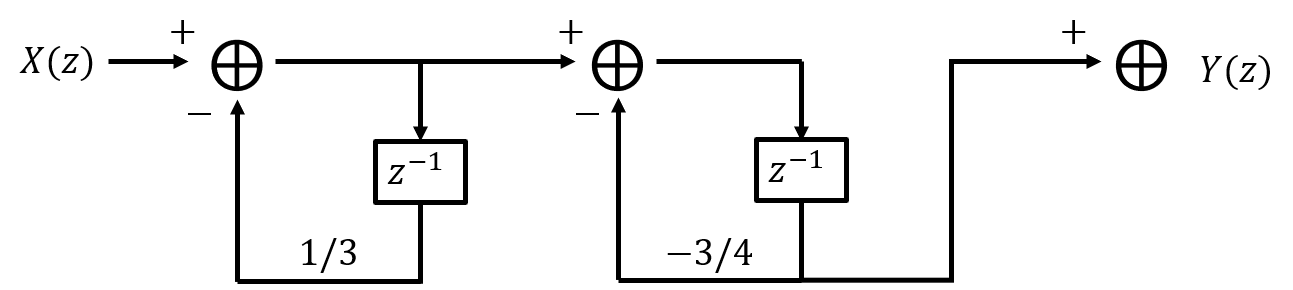
\includegraphics[width=12cm]{cascade_form_block.png}}
\end{figure}

\item[(b)]{Classify the frequency responses in the figure as being lowpass, highpass or bandstrop.}

\begin{figure}[h!]
\center{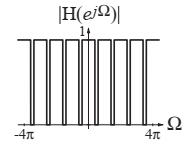
\includegraphics[width=5cm]{problem2b.png}}
\end{figure}

\textbf{Solution:} \\
This is a frequency reponse of a \textbf{bandstop filter}. The transfer function can be represented as
\begin{equation}
H(e^{j\Omega}) = A e^{-j\Omega n_{0}} \left\lbrace 1 - \left[ \mathtt{rect}\left(\frac{\Omega - \Omega_{0}}{\Delta \Omega} \right) + \mathtt{rect} \left(\frac{\Omega - \Omega_{0}}{\Delta\Omega} \right) \right] \ast \delta_{2 \pi}(\Omega) \right\rbrace
\end{equation}

\pagebreak
\item[(c)]{Calculate the filter responses of the following FIR filter.}
\begin{equation}
h_{N}[n] = \sum_{m=0}^{N-1}{a_{m} \delta[n - m]},
\end{equation}
where $N = 0$, $a_{0} = 0.25$, $a_{1} = 0.50$, $a_{2} = 0.25$.
\end{itemize}

\begin{itemize}
\item[1.]{Impulse response}

\begin{equation}
\begin{gathered}
\begin{alignedat}{1}
h_{N}[n] &= a_{0}\delta[n] + a_{1}\delta[n-1] + a_{2}\delta[n-2] \\
h_{N}[n] &= 0.25\delta[n] + 0.50\delta[n-1] + 0.25\delta[n-2]
\end{alignedat}
\end{gathered}
\end{equation}

\begin{figure}[h!]
\center{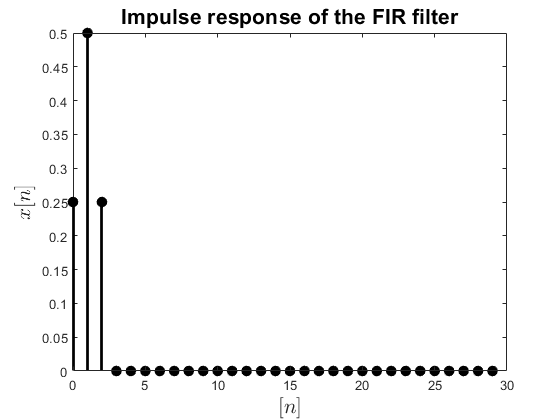
\includegraphics[width=11cm]{prob2c_1.png}}
\end{figure}

\item[2.]{Excitation: \{..., 0, 0, 8, 8, 8, 0, 0, ...\}}

\begin{figure}[h!]
\center{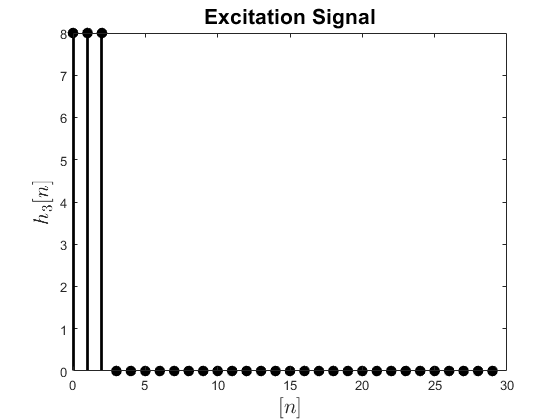
\includegraphics[width=11cm]{prob2c_2.png}}
\end{figure}

\pagebreak

\begin{figure}[h!]
\center{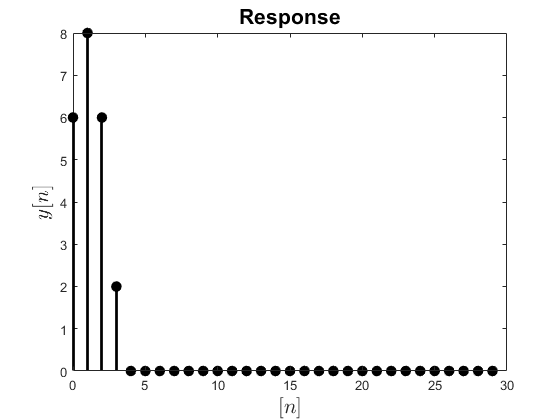
\includegraphics[width=11cm]{prob2c_3.png}}
\end{figure}
\end{itemize}

\item[\textbf{(3)}]{\textbf{MATLAB coding.}}
Design the FIR filters to separate do, mi, sol from do-mi-sol chord, respectively.
\begin{itemize}
\item{Source code}
\item{Filter coefficients for do, mi, sol, respectively}
\item{Plot the Bode diagram of the designed filter}
\item{Attach the output MP3 files of the designed filters}
\end{itemize}

\pagebreak
\begin{tcolorbox}[enforce breakable, pad at break = 1mm, break at=25cm,title={Source Code}]
\lstinputlisting[language=Matlab, upquote=true]{prob3.m}
\end{tcolorbox}

\textbf{Bode diagram of the designed filter for do:}
\begin{figure}[h!]
\center{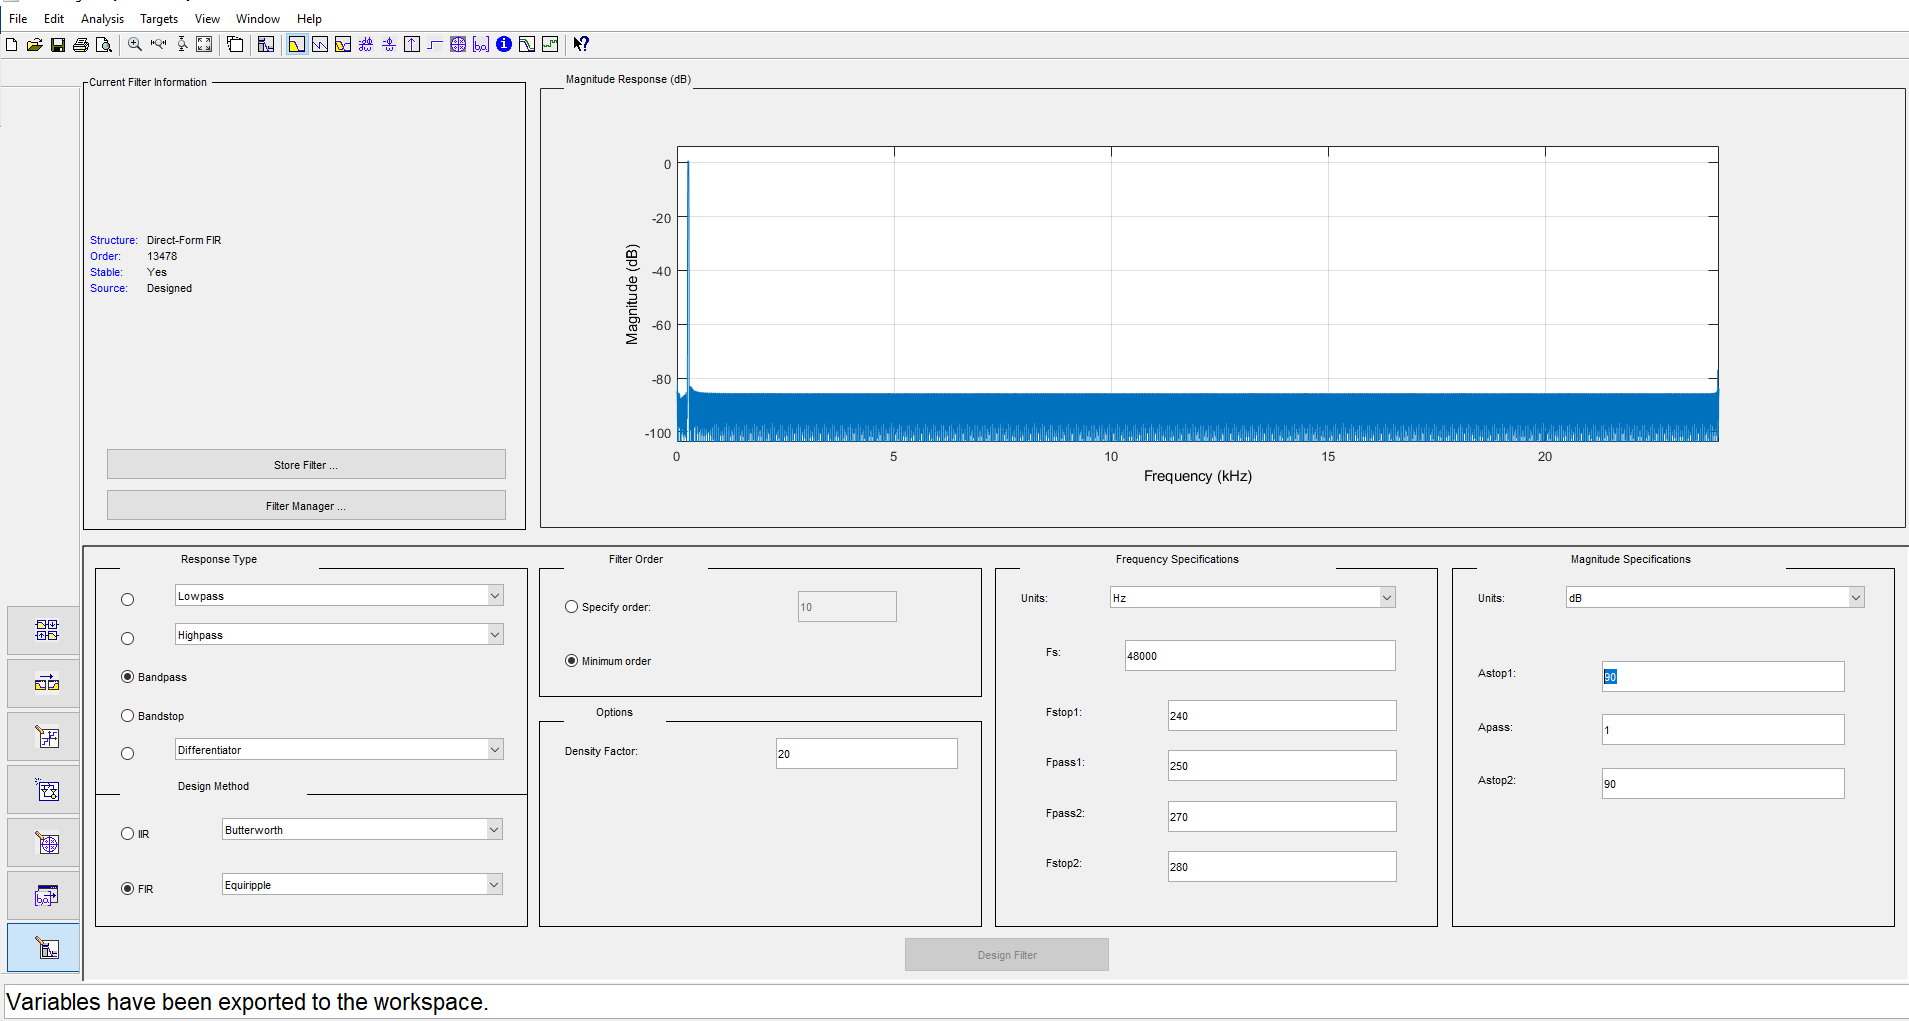
\includegraphics[width=13cm]{filter_do.png}}
\end{figure}

\pagebreak
\textbf{Bode diagram of the designed filter for mi:}
\begin{figure}[h!]
\center{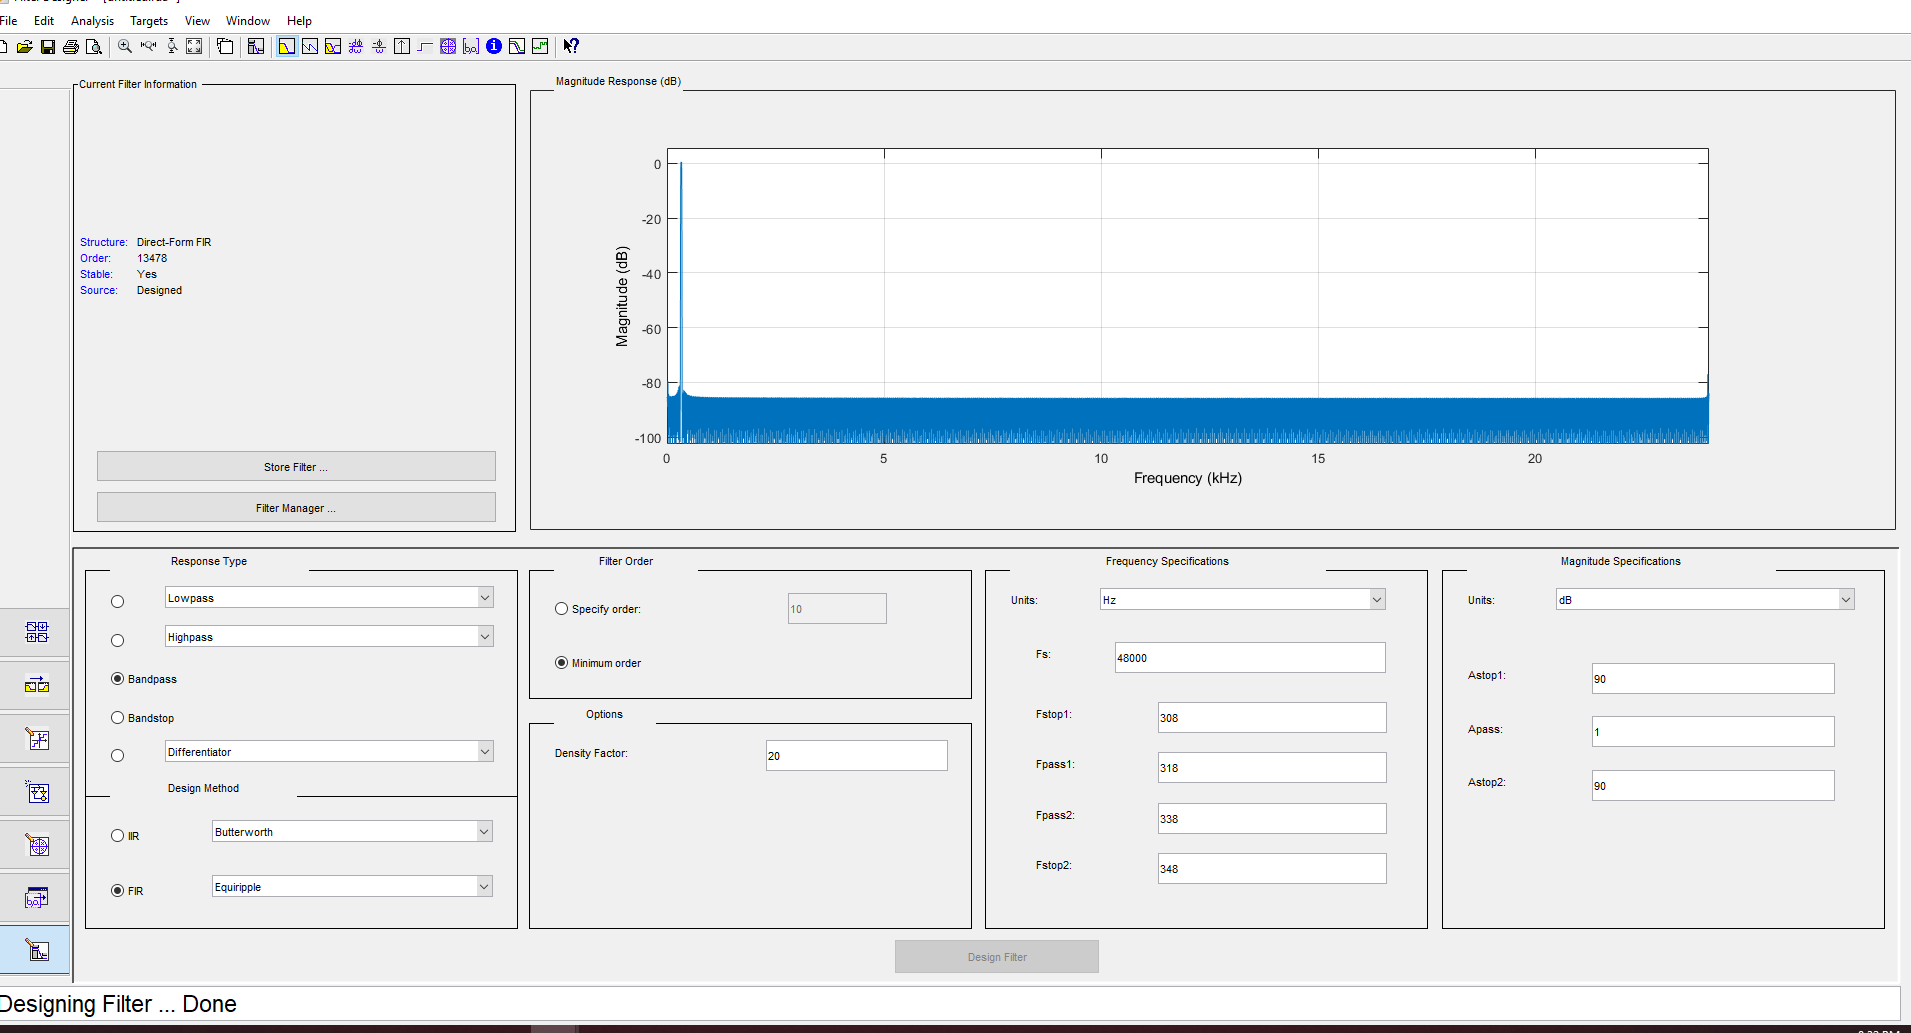
\includegraphics[width=13cm]{filter_mi.png}}
\end{figure}

\textbf{Bode diagram of the designed filter for so:}
\begin{figure}[h!]
\center{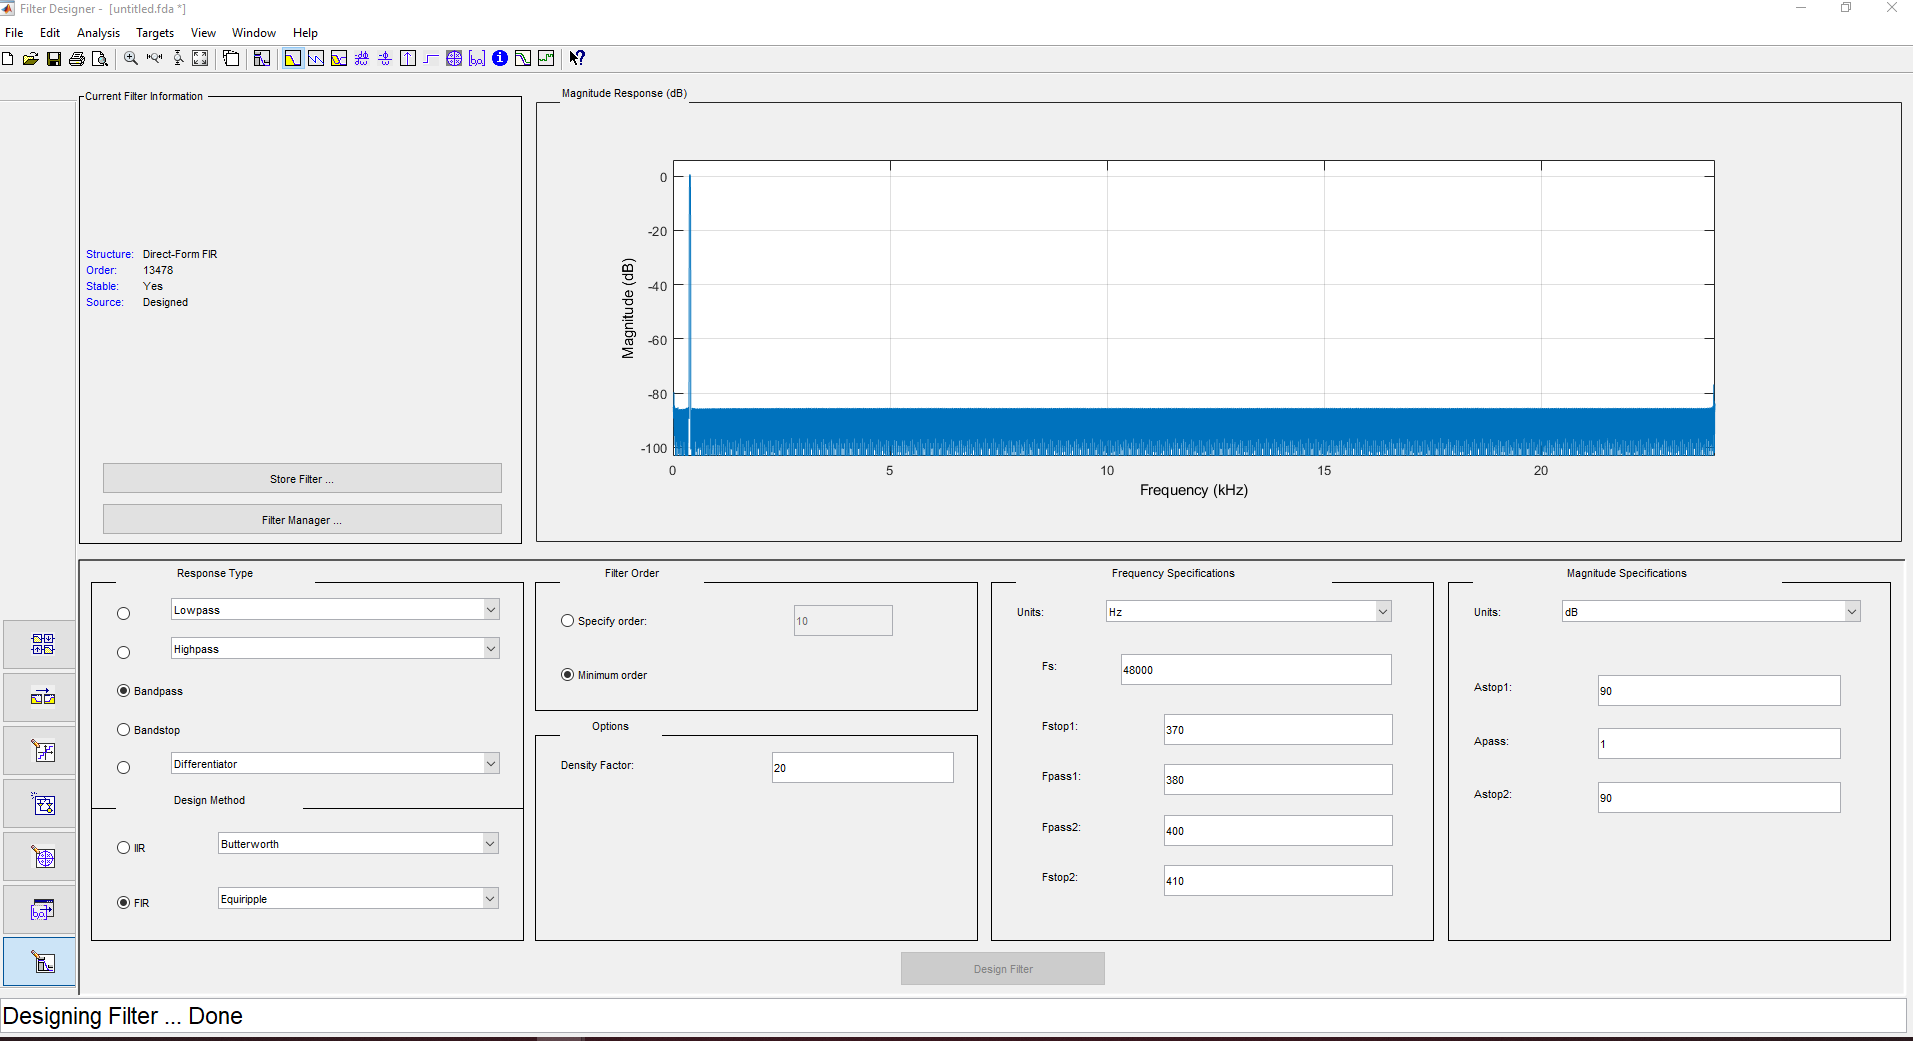
\includegraphics[width=13cm]{filter_so.png}}
\end{figure}

\vspace{2cm}
\begin{tcolorbox}[title={\textbf{Note: All the files were uploaded on GitHub}}]
All the files in this document were uploaded on Github, and can be accessed at:


\begin{center}
\url{https://github.com/rjcanoy03/BRI509/tree/Assignment%233}
\end{center}


If there are errors in the solution or codes kindly email, $\\$
recanoy@korea.ac.kr.
\end{tcolorbox}
\end{itemize}
\end{document}